\documentclass[a4paper,12pt]{report}

% Regolazione margini
\usepackage{geometry}
\geometry{a4paper, top=1.9cm, bottom=2cm, left=2cm, right=2cm}

\usepackage{alltt, fancyvrb, url}
\usepackage{graphicx}
\usepackage[utf8]{inputenc}
\usepackage{hyperref}
\usepackage{float}

\usepackage[italian]{babel}

\usepackage[italian]{cleveref}

% Grafica e personalizzazione
\usepackage{graphicx}
\usepackage{booktabs}
\usepackage{keyval}
\usepackage{sidecap}
\usepackage{caption}
\usepackage{wrapfig}
\usepackage{floatflt}
\usepackage{imakeidx}
\usepackage{amssymb}
\usepackage{wasysym}
\usepackage[dvipsnames,usenames]{xcolor}
\usepackage{tikz}

% Per mostrare codice
\usepackage{listings}
\lstset{
	language=SQL,
	basicstyle=\footnotesize\ttfamily,
	keywordstyle=\color{black}\bfseries,
	commentstyle=\color{darkgray},
	stringstyle=\color{black},
	stepnumber = 1,                  		% the step between two line-numbers.
	numbersep = 5pt,                        % how far the line-numbers are from the 
	tabsize=4,
	frame=tb,								% adds a frame around the code
	showspaces = false,                     % show spaces adding particular 
	showstringspaces = false,               % underline spaces within strings
	showtabs = false,                       % show tabs within strings adding 
	numberstyle = \scriptsize\bf\color{lightgray}, 
	backgroundcolor = \color{lightgray!50},
	rulecolor = \color{lightgray},
	keywordstyle = \bfseries\color{blue!80},	
	framexleftmargin = 0mm,
	numberblanklines = false,
	xleftmargin = 5pt,
	breaklines = true,
	breakatwhitespace = true,
	breakautoindent = true,
	captionpos = t,
	texcl = true,
	tabsize = 3,                            % sets default tabsize to 3 spaces
	extendedchars = true,
	inputencoding = utf8, 
	escapechar = \à,
	% more key words to emphasize
	morekeywords={print, println, size, background, strokeWeight, fill, line, rect, ellipse, triangle, arc, save, PI, HALF_PI, QUARTER_PI, TAU, TWO_PI, width, height},	
	emph={[1]print,println},emphstyle={[1]\bf\color{blue}},
	emph={[2]for,while},emphstyle={[2]\bf\color{ForestGreen}},
	emph={[3]case},emphstyle={[3]\bf\color{violet}},
	}

% Colorare e modificare le tabelle
\usepackage{array}
\newcolumntype{L}[1]{>{\raggedright\arraybackslash}p{#1}}
\newcolumntype{C}[1]{>{\centering\arraybackslash}p{#1}}
\newcolumntype{R}[1]{>{\raggedleft\arraybackslash}p{#1}}
\usepackage{colortbl}
\usepackage{multirow}
%tabella senza linee 
\newcommand{\quantities}[1]{ %serve per inserire dati nella tabella   
	\begin{tabular}{@{}c@{}}\strut#1\strut\end{tabular}%
}

\title{\textbf{DB-Garage}\\Relazione per\\``Elaborato di Basi di Dati''}

\author{Barberini Elisa\\Mainardi Giosuè Giocondo}
\date{\today}

\begin{document}

\maketitle

\tableofcontents

\chapter{Analisi dei requisiti}
L'autofficina \textbf{DB-Garage}$^{\copyright}$ richiede la realizzazione di un database per la gestione di automobili,
%
clienti, dipendenti e delle loro interazioni, ovvero riparazioni e acquisto o vendita di veicoli, nuovi o usati. Vengono di seguito 
%
descritti gli aspetti caratterizzanti del dominio.

\section{Intervista}

Di ogni utente del portale (cliente o impiegato) è necessario memorizzare: codice fiscale, nome, cognome,
%
data di nascita e telefono. Si può inoltre aggiungere, preferibilmente, anche una e-mail per le eventuali comunicazioni. 
%
La mail e il telefono di ogni persona devono poter essere aggiornati nel caso in cui il contatto del cliente o dell'impiegato cambi.
%
I dipendenti si differenziano in base al tipo di attività che possono svolgere, che può essere quello di riparazioni o 
%
quello di compravendita.
%
Il primo tipo di lavoratori è formato da meccanici ed il secondo da agenti automobilistici, di entrambi si vuole memorizzare 
%
anche la retribuzione oraria, che deve poter essere aggiornata, in caso di modifiche contrattuali.

Le automobili appartengono tutte a una casa produttrice, hanno un modello, una cilindrata e un anno di produzione.
%
In aggiunta, le auto usate hanno già la targa, univoca, e, avendo già circolato prima dell'inserimento in officina, 
%
occorre tener conto dei km percorsi ed eventualmente aggiornarli.
%
Ciascun veicolo può essere oggetto di molteplici attestati di proprietà con il suo cliente proprietario, 
%
ma un auto potrà avere solo un attestato non scaduto, altrimenti vorrà dire che è di proprietà dell'officina.

Le riparazioni sono relative alle automobili usate, hanno un costo totale concordato con il cliente, coinvologono
%
uno o più meccanici e in caso utilizzano anche dei pezzi di ricambio.

Per avere una panoramica della qualità dei marchi di automobili, i meccanici ritengono utile avere la lista delle 
%
case produttrici i cui veicoli hanno avuto più di 10 riparazioni nell'ultimo anno.

Inoltre per tenere traccia dei lavoratori con più esperienza o qualità, si vuole stilare la classifica dei 5 meccanici
%
più laboriosi in ordine di n° di riparazioni effettuate in totale dall'apertura dell'officina.

Il sistema deve considerare gli eventuali pezzi di ricambio utilizzati che sono individuati dalla targa del veicolo di
%
riferimento e dal nome, con l'aggiunta del costo unitario e una breve descrizione se necessaria.

Ogni transazione nel reparto compravendita viene effettuata da un agente automobilistico con un cliente 
%
e riguarda uno specifico veicolo, di essa si vogliono memorizzare se sia acquisto(l'officina compra l'auto 
%
dal un cliente) o vendita(l'officina vende l'auto ad un cliente), prezzo concordato e la data. 
% 
Una transazione, una volta effettuata, determinerà un passaggio di proprietà del veicolo in oggetto

L'officina vuole premiare gli agenti meritevoli e quindi deve essere possibile ottenere il venditore che ha fatto
%
più transazioni in uno specifico mese. 

La base di dati deve mantenere in memoria sia la data di inizio che la data di fine di ogni riparazione effettuata
% 
(inserite manualmente), di ogni transazione e di ogni attestato di proprietà (in base alla data di inserimento),
%
così da poter essere mostrati in caso di richiesta dai clienti.

\section{Tabella concetti principali con sinonimi e definizioni}

\begin{figure}[H]
	\fontsize{10pt}{12pt}\selectfont
	\advance\leftskip-4cm
	\centering
	\arrayrulecolor{BlueGreen}
	\begin{tabular}{l c c }
		\rowcolor{BlueGreen}
		\rule[-3mm]{0mm}{0.85cm}
		\textbf{Termine} & \textbf{Eventuali sinonimi} &\textbf{Breve descrizione} \\
		\hline\rule[-3mm]{0mm}{0.85cm}
		Utente & Persona & \quantities{Persona registrata nel sistema.} \\
		\hline\rule[-3mm]{0mm}{0.85cm}
		Dipendente & \quantities{Impiegato, Lavoratore} & \quantities{Persona che lavora per l'officina \\come meccanico o agente.} \\
		\hline\rule[-3mm]{0mm}{0.85cm}
		Cliente & & \quantities{Persona che deve eseguire o ha eseguito una \\riparazione o una transazione con l'officina. }\\
		\hline\rule[-3mm]{0mm}{0.85cm}
		Meccanico & & \quantities{Dipendente dell'officina che esegue riparazioni.} \\
		\hline\rule[-3mm]{0mm}{0.85cm}
		Agente & \quantities{Agente automobilistico, Venditore} & \quantities{Dipendente dell'officina che esegue transazioni.}\\
		\hline\rule[-3mm]{0mm}{0.85cm}
		Riparazione & Lavoro & \quantities{Servizio di uno o più meccanici riguardo a un \\veicolo, su richiesta di un cliente.}\\
		\hline\rule[-3mm]{0mm}{0.85cm}
		Transazione & & \quantities{Servizio di un agente per l'acquisto o la \\vendita di un auto da parte di un cliente.}\\
		\hline\rule[-3mm]{0mm}{0.85cm}
		Veicolo & \quantities{Auto, \\ Automobile} & Oggetto dei servizi dell'officina.  \\
		\hline\rule[-3mm]{0mm}{0.85cm}
		Attestato & Attestato di proprietà & \quantities{Documento che certifica l'appartenenza di \\un auto ad una determinata persona.} \\
		\hline\rule[-3mm]{0mm}{0.85cm}
		Acquisto &  & \quantities{Transazione che determina il passaggio di \\proprietà di un auto da un cliente all'officina.} \\
		\hline\rule[-3mm]{0mm}{0.85cm}
		Vendita &  & \quantities{Transazione che determina il passaggio di \\proprietà di un auto dall'officina ad un cliente.} \\
		\hline\rule[-3mm]{0mm}{0.85cm}
		Pezzo di ricambio &  & \quantities{Articolo che può essere necessario \\per la riparazione di un auto.} \\
		\hline
	\end{tabular}
\end{figure}
\section{Definizione specifiche in linguaggio naturale}
L'autofficina \textbf{DB-Garage}$^{\copyright}$ richiede la realizzazione di un database per la gestione di automobili,
%
clienti, dipendenti e delle loro interazioni, ovvero riparazioni e acquisto o vendita di veicoli, nuovi o usati. Vengono di seguito 
%
descritti gli aspetti caratterizzanti del dominio.

Un \textbf{Utente} è una persona registrata nel sistema della quale è necessario memorizzare: codice fiscale, nome, cognome,
%
data di nascita e telefono, più una e-mail opzionale. Telefoo e E-mail devono essere aggiornabili.

Un \textbf{Cliente} è una semplice sottoclasse di Utente senza attributi aggiuntivi, che ha effettuato o deve effettuare 
%
una Riparazione o una Transazione.

\textbf{Dipendente} è un'altra sottoclasse ma che ha anche una paga oraria, aggiornabile, e due sottoclassi a sua volta: \textbf{Meccanico} e \textbf{Agente}.

L'oggetto principale delle operazioni del sistema è il \textbf{Veicolo} che è identificato da modello, casa produttrice, cilindrata e anno di produzione.
%
I veicoli possono essere nuovi o usati, quelli usati sono identificati univocamente dalla targa e inoltre ne vengono 
%
memorizzati anche i km percorsi, quest'ultimo attributo deve poter essere aggiornato.
%
Ciascun Veicolo può essere oggetto di molteplici \textbf{Attestati} con il suo \underline{Utente proprietario}, 
%
ma un Veicolo potrà avere solo un Attestato non scaduto, altrimenti vorrà dire che è di proprietà dell'\textit{Officina}.

Le \textbf{Riparazioni} sono relative solo ai Veicoli \underline{usati}, hanno un costo totale, coinvologono uno o più 
%
\textbf{Meccanici} e opzionalmente dei pezzi di ricambio.

L'\textit{Officina} ritiene utile avere una \underline{Lista delle case produttrici} i cui veicoli hanno avuto più di 10 riparazioni
%
nell'ultimo anno e la \underline{Classifica di 5 Meccanici} in ordine di n° di riparazioni effettuate in totale.

Inoltre, il sistema deve considerare gli eventuali \textbf{Pezzi di ricambio} utilizzati che sono individuati da 
%
targa e nome, con l'aggiunta del costo unitario e una breve descrizione, opzionale.

Ogni \textbf{Transazione} viene effettuata da un \textbf{Agente} con un \textbf{Cliente} e riguarda un specifico \textbf{Veicolo},
%
di essa si vuole memorizzare se sia acquisto(l'\textit{Officina} compra l'auto dall'Utente) o vendita(l'\textit{Officina} 
% 
vende l'auto ad un Utente), prezzo e data. 

\noindent
Una Transazione determina un passaggio di proprietà del Veicolo in oggetto, quindi il relativo \textbf{Attestato} 
%
dovrà essere posto come scaduto e ne sarà inserito un altro se il Veicolo passa ad un Cliente(\underline{Transazione di Vendita}),
%
mentre se passa all'\textit{Officina}(\underline{Transazione di Acquisto}) no.

Deve essere possibile ottenere l' \underline{Agente del mese}, cioè quello con più transazioni in un dato periodo. 

Devono essere tenute in memoria sia la data di inizio che la data di fine di ogni Riparazione effettuata, inserite manualmente,
%
invece per ogni Transazione e Attestato, va registrata la data di inserimento.

\subsection*{Principali azioni richieste:}
\begin{enumerate}
	\item Inserimento cliente
	\item Inserimento veicolo usato
	\item Inserimento riparazione
	\item Vendita veicolo nuovo
	\item Acquisto veicolo usato 
	\item Visualizza elenco clienti
	\item Visualizza elenco veicoli nuovi
	\item Visualizza elenco veicoli dei clienti
	\item Visualizza elenco veicoli usati in vendita 
	\item Visualizza le case produttrici più carenti dell'anno 
	\item Visualizza i 5 meccanici più laboriosi
	\item Ottieni l'agente del mese
	\item Aggiorna attributo scaduto su atto di proprietà
	\item Aggiorna attributo e-mail
	\item Aggiorna attributo km percorsi in veicoli usati 
\end{enumerate}

\chapter{Progettazione Concettuale}

\section{Schema Scheletro}
\addcontentsline{toc}{section}{Schema Scheletro}	
	\begin{figure}[H]
		\centering
		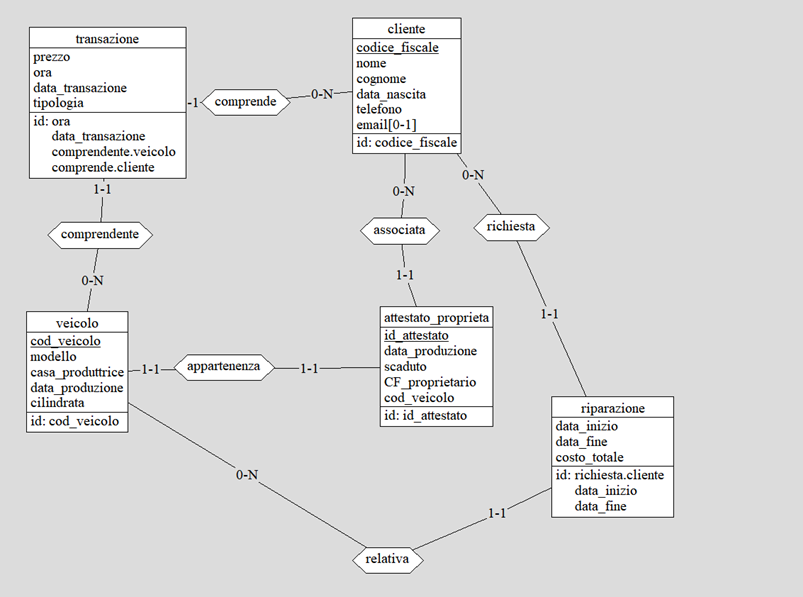
\includegraphics[scale=1]{img/schema_scheletro.png}
	\end{figure}

\section{Raffinamenti proposti}
L’entità più importante da individuare inizialmente è cliente identificato dal suo codice fiscale.

Tuttavia, all’interno dell’officina non devono essere memorizzati solo i clienti ma anche i dipendenti divisi tra agenti e meccanici.

Proprio per questo si è deciso di creare un’entità generica persona, contenente tutte le loro informazioni da cui dar luogo ad una
%
gerarchia che definisce ogni tipo di individuo che ha a che fare con l’officina.

Questa gerarchia viene utilizzata poiché i vari ruoli partecipano alle relative associazioni con semantiche differenti(infatti, un
%
agente svolge solo transazioni di compravendita mentre un meccanico si occupa solo delle riparazioni).

La mail è un attributo opzionale in quanto come recapito obbligatorio vi è già il numero di telefono, inoltre potrebbe essere utile al 
%
cliente nel caso decidesse di ricevere notizia dell’operazione che si sta svolgendo (transazione o riparazione) tramite canali digitali.

Essendo che sia agente che meccanico hanno in comune l’attributo paga oraria che cliente non ha risulta utile definire la gerarchia
%
dipendente.

Risulterà importante conoscere i dati dell’utente per permettere la storicizzazione delle operazioni di compravendita e riparazione 
%
dei vari veicoli.

A tal scopo, è necessario individuare l’entità veicolo, entità fondamentale per l’officina.

I veicoli possono essere usati o nuovi, ciò che differenzia le due tipologie è che i veicoli usati hanno due attributi aggiuntivi, 
%
ovvero i km percorsi e la targa.

\addcontentsline{toc}{section}{Raffinamenti}	
	\begin{figure}[H]
		\centering
		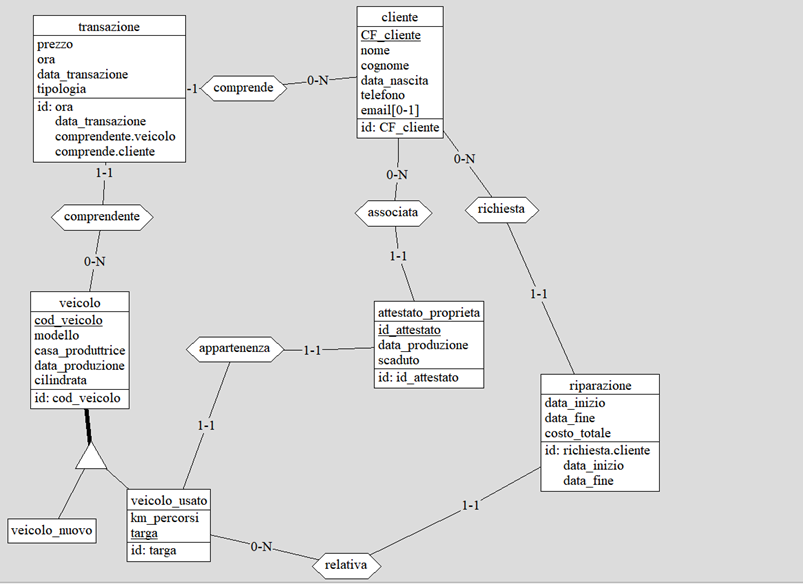
\includegraphics[scale=1]{img/raffinamenti.png}
	\end{figure}

I veicoli nuovi sono identificati da un codice mentre i veicoli usati dalla targa.

Possono essere presenti più veicoli nuovi od usati con stessa casa produttrice, stesso modello, stessa cilindrata ed uguale anno di produzione.

Si sottolinea che per ciascun veicolo usato la targa deve essere unica.

Data l’introduzione di due tipologie di veicolo si vede, quindi, l’esigenza di introdurre la gerarchia veicolo, dato che veicoli 
%
nuovi ed usati partecipano differentemente alle varie operazioni ed associazioni.

Sia veicoli usati che nuovi possono essere venduti ed acquistati. un veicolo nuovo una volta venduto ad un cliente diventa usato 
%
con km percorsi pari a 0.

Una volta che un veicolo nuovo viene venduto esso diventa usato con km percorsi pari a 0 e prevede l’inserimento di una targa.

Ogni veicolo usato deve avere un proprietario ed uno e uno solo attestato di proprietà.

Un cliente può essere proprietario di più veicoli usati ma ogni veicolo può e deve avere uno e uno solo attestato di proprietà, 
%
ovvero un solo proprietario. 

Il proprietario del veicolo può essere un cliente registrato o l’officina stessa e viene indicato tramite l’attributo scaduto 
%
dell’entità attestato di proprietà che può assumere due differenti valori ovvero 0 e 1.

Se l’attributo scaduto ha valore 1 significa che il veicolo è stato acquistato dall’officina che ne risulta quindi proprietaria, 
%
in caso contrario il proprietario del veicolo è il cliente registrato con codice fiscale uguale a quello dell’attestato.

Ogni transazione di compravendita vede come protagonisti un cliente e un agente, l’officina può comprare i veicoli usati dai clienti 
%
mentre i clienti possono comprare i veicoli nuovi o usati di proprietà dell’officina.

La transazione è individuata da cliente, veicolo ora e data.

Ogni agente può effettuare più transazioni di acquisto o vendita.

Risulta importante sottolineare che ogni qualvolta un determinato veicolo viene sottoposto ad una transazione, sia essa di vendita o 
%
acquisto, da parte dell’officina l’attestato di proprietà corrispondente viene aggiornato.

Ogni automobile usata può essere sottoposta a riparazioni che vengono effettuate da uno o più meccanici e che interessano uno o più 
%
pezzi di ricambio.

Se all’interno di una riparazione si vogliono utilizzare dei pezzi di ricambio questi devono prima essere registrati con nome, 
%
descrizione opzionale e selezionando un veicolo di riferimento scelto tra quelli già presenti nel sistema.

Ogni riparazione è individuata dal cliente a cui è riferita il veicolo la data di inizio e la data di fine.

Uno stesso veicolo usato può ricevere un numero indeterminato di riparazioni anche da parte dello stesso meccanico.

Un cliente può richiedere più riparazioni ma non vi possono essere più riparazioni registrate per un determinato cliente ad uno 
%
specifico veicolo con data di inizio e di fine della riparazione corrispondenti.

\section{Schema Finale}
\addcontentsline{toc}{section}{Schema Finale}	
	\begin{figure}[H]
		\centering
		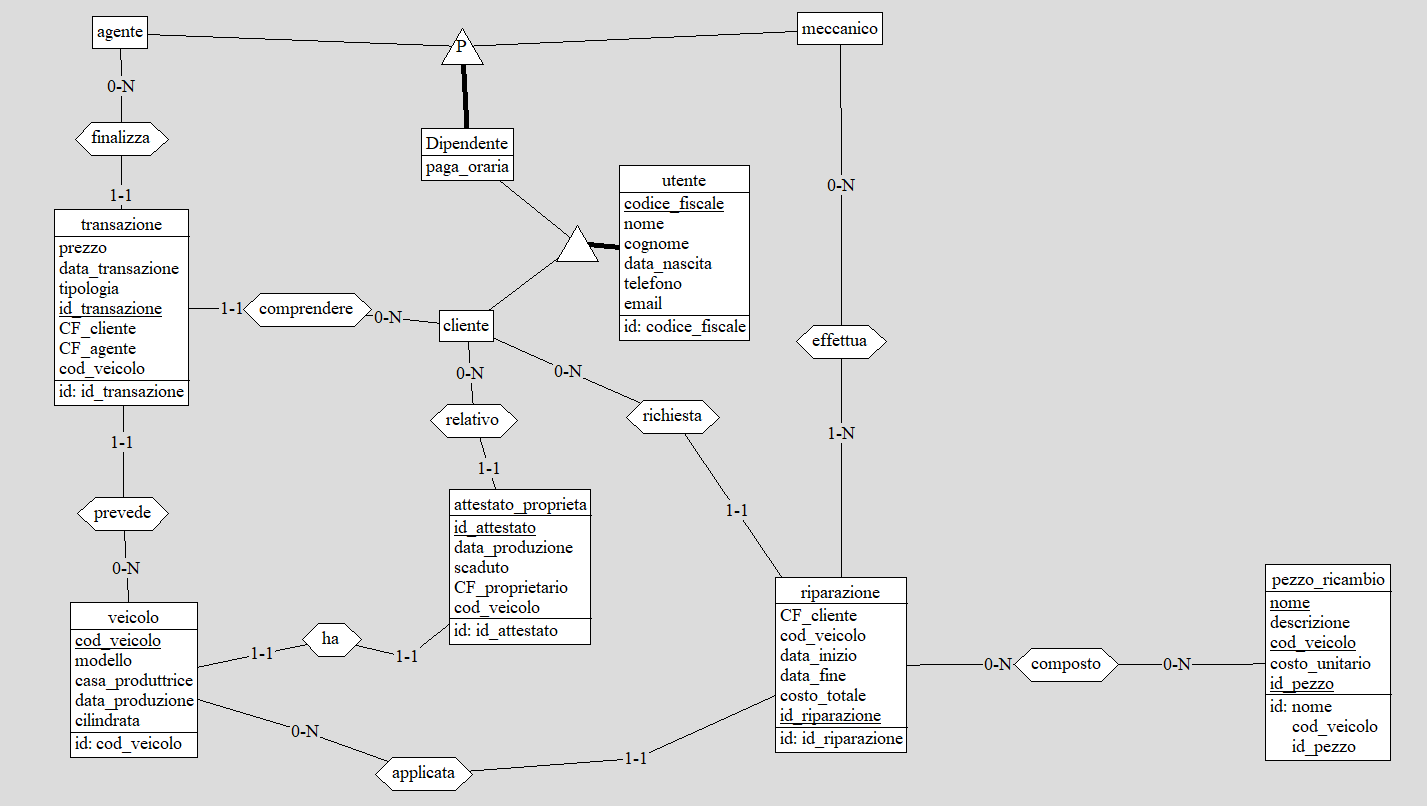
\includegraphics[scale=1]{img/schema_finale.png}
	\end{figure}

\chapter{Progettazione Logica}

\section{Stima Volume dati}
\begin{figure}[H]
	\fontsize{14pt}{12pt}\selectfont
	\advance\leftskip-15cm
	\centering
	\arrayrulecolor{BlueGreen}
	\begin{tabular}{l c c }
		\rowcolor{BlueGreen}
		\rule[-3mm]{0mm}{0.85cm}
		\textbf{Concetto} & \textbf{Costrutto} &\textbf{Volume} \\
		\hline\rule[-2mm]{0mm}{0.75cm}
		Utente & E & 3050\\
		\hline\rule[-2mm]{0mm}{0.75cm}
		Cliente & E & 3000 \\
		\hline\rule[-2mm]{0mm}{0.75cm}
		Dipendente & E & 50\\
		\hline\rule[-2mm]{0mm}{0.75cm}
		Agente & E & 20\\
		\hline\rule[-2mm]{0mm}{0.75cm}
		Meccanico & E & 30\\
		\hline\rule[-2mm]{0mm}{0.75cm}
		Possesso & R & 6000 \\
		\hline\rule[-2mm]{0mm}{0.75cm}
		Attestato & R & 6000\\
		\hline\rule[-2mm]{0mm}{0.75cm}
		Riguardo & R & 6000 \\
		\hline\rule[-2mm]{0mm}{0.75cm}
		Veicolo & E & 6120 \\
		\hline\rule[-2mm]{0mm}{0.75cm}
		Veicolo Nuovo & E & 120 \\
		\hline\rule[-2mm]{0mm}{0.75cm}
		Veicolo Usato & E & 6000 \\
		\hline\rule[-2mm]{0mm}{0.75cm}
		Coinvolgimento & R & 1000\\
		\hline\rule[-2mm]{0mm}{0.75cm}
		Transazione & R & 1000\\
		\hline\rule[-2mm]{0mm}{0.75cm}
		Transazione d'acquisto& R & 400\\
		\hline\rule[-2mm]{0mm}{0.75cm}
		Transazione di vendita& R & 600\\
		\hline\rule[-2mm]{0mm}{0.75cm}
		Perseguimento & R & 1000\\
		\hline\rule[-2mm]{0mm}{0.75cm}
		Esecuzione & R & 1000\\
		\hline\rule[-2mm]{0mm}{0.75cm}
		Lavorazione & R & 12000\\
		\hline\rule[-2mm]{0mm}{0.75cm}
		Riparazione & E & 12000\\
		\hline\rule[-2mm]{0mm}{0.75cm}
		Richiesta & R & 12000\\
		\hline\rule[-2mm]{0mm}{0.75cm}
		Sottoposizione & R & 12000\\
		\hline\rule[-2mm]{0mm}{0.75cm}
		Utilizzo & R & 15000\\
		\hline\rule[-2mm]{0mm}{0.75cm}
		Pezzo di ricambio & E &  9000\\
		\hline
	\end{tabular}
\end{figure}

\section{Descrizione operazioni principali e stima frequenza}
\begin{figure}[H]
	\fontsize{14pt}{12pt}\selectfont
	\advance\leftskip-15cm
	\centering
	\arrayrulecolor{BlueGreen}
	\begin{tabular}{c c c }
		\rowcolor{BlueGreen}
		\rule[-6mm]{0mm}{1.5cm}
		\textbf{Codice} & \textbf{Operazione} &\textbf{Frequenza} \\
		\hline\rule[-5mm]{0mm}{1.4cm}
		1 & Inserimento cliente & 8 al giorno \\
		\hline\rule[-5mm]{0mm}{1.4cm}
		2 & Inserimento veicolo usato & 10 al giorno \\
		\hline\rule[-5mm]{0mm}{1.4cm}
		3 & Inserimento riparazione & 18 al giorno \\
		\hline\rule[-5mm]{0mm}{1.4cm}
		4 & Vendita veicolo nuovo & 3 a settimana \\
		\hline\rule[-5mm]{0mm}{1.4cm}
		5 & Acquisto veicolo usato & 8 a settimana \\
		\hline\rule[-5mm]{0mm}{1.4cm}
		6 & Visualizza elenco clienti & 25 al giorno \\
		\hline\rule[-5mm]{0mm}{1.4cm}
		7 & Visualizza elenco veicoli nuovi & 10 al giorno \\
		\hline\rule[-5mm]{0mm}{1.4cm}
		8 & Visualizza elenco veicoli dei clienti & 28 al giorno \\
		\hline\rule[-5mm]{0mm}{1.4cm}
		9 & \quantities{Visualizza elenco veicoli\\usati in vendita} & 12 al giorno  \\
		\hline\rule[-5mm]{0mm}{1.4cm}
		10 & \quantities{Visualizza le case produttrici\\più carenti dell'anno} & 1 all'anno  \\
		\hline\rule[-5mm]{0mm}{1.4cm}
		11 & \quantities{Visualizza i 5 meccanici\\più laboriosi} & 1 al giorno \\
		\hline\rule[-5mm]{0mm}{1.4cm}
		12 & Visualizza l'agente del mese & 1 al mese \\
		\hline\rule[-5mm]{0mm}{1.4cm}
		13 & Aggiorna attributo e-mail & 5 a settimana \\
		\hline\rule[-5mm]{0mm}{1.4cm}
		14 & \quantities{Aggiorna attributo km percorsi\\in veicoli usati} & 1 alla settimana \\
		\hline
	\end{tabular}
\end{figure}
\newpage
\section{Schemi di navigazione e tabelle accessi}
\subsection*{Operazione 1: Inserimento cliente}
\begin{figure}[H]
	\centering
	\arrayrulecolor{BlueGreen}
	\begin{tabular}{L{3cm}C{2cm}C{4.5cm}C{2cm}}
		\rowcolor{BlueGreen}\rule[-1.5mm]{0mm}{0.60cm}{}
		\textbf{Concetto} & \textbf{Costrutto} &\textbf{Accessi} & \textbf{Tipo} \\	
		\hline\rule[-2mm]{0mm}{0.65cm}{}
		Cliente & E & 1 & S \\
	\end{tabular}
	
	\begin{tabular}{C{12.9cm}}
		\rule[-3mm]{0mm}{0.85cm}{}	
		\cellcolor{BlueGreen} \textbf{\underline{Totale:} 1 S $\to$ 2 x 8 = 16 accessi al giorno}
	\end{tabular}
\end{figure}

\subsection*{Operazione 2: Inserimento veicolo usato}
\begin{figure}[H]
	\centering
	\arrayrulecolor{BlueGreen}
	\begin{tabular}{L{3cm}C{2cm}C{4.5cm}C{2cm}}
		\rowcolor{BlueGreen}\rule[-2mm]{0mm}{0.6cm}{}
		\textbf{Concetto} & \textbf{Costrutto} &\textbf{Accessi} & \textbf{Tipo} \\
		\hline\rule[-2mm]{0mm}{0.65cm}{}
		Cliente & E & 3 000 & L \\
		\hline\rule[-2mm]{0mm}{0.65cm}{}
		Veicolo Usato & E & 1 & S \\
		\hline\rule[-2mm]{0mm}{0.65cm}{}
		Attestato & R & 1 & L \\
	\end{tabular}
	
	\begin{tabular}{C{12.9cm}}
		\rule[-3mm]{0mm}{0.85cm}{}	
		\cellcolor{BlueGreen} \textbf{\underline{Totale:} 1 S + 3 001 L $\to$ 3 003 x 10 = 30 030 accessi al giorno}
	\end{tabular}
\end{figure}

\subsection*{Operazione 3: Inserimento riparazione}
\begin{figure}[H]
	\centering
	\arrayrulecolor{BlueGreen}
	\begin{tabular}{L{3.7cm}C{2.2cm}C{4.7cm}C{2cm}}
		\rowcolor{BlueGreen}\rule[-2mm]{0mm}{0.6cm}{}
		\textbf{Concetto} & \textbf{Costrutto} &\textbf{Accessi} & \textbf{Tipo} \\
		\hline\rule[-2mm]{0mm}{0.65cm}{}
		Cliente & E & 3 000 & L \\
		\hline\rule[-2mm]{0mm}{0.65cm}{}
		Attestato & R & 3 000 & L \\
		\hline\rule[-2mm]{0mm}{0.65cm}{}
		Cliente & E & 1 & L \\
		\hline\rule[-2mm]{0mm}{0.65cm}{}
		Veicolo Usato & E & 6 000 / 3 000 = 2 & L \\
		\hline\rule[-2mm]{0mm}{0.65cm}{}
		Veicolo Usato & E & 1 & L \\
		\hline\rule[-2mm]{0mm}{0.65cm}{}
		Meccanico & E & 30 & L \\
		\hline\rule[-2mm]{0mm}{0.65cm}{}
		Pezzo di ricambio & E & 9 000 / 6 000 = 1,5 & L \\
		\hline\rule[-2mm]{0mm}{0.65cm}{}
		Riparazione & E & 1 & S \\
		\hline\rule[-2mm]{0mm}{0.65cm}{}
		Riparazione & E & 1 & L \\
		\hline\rule[-2mm]{0mm}{0.65cm}{}
		Lavorazione & R & 1 & S \\
		\hline\rule[-2mm]{0mm}{0.65cm}{}
		Utilizzo & R & 1 & S \\
	\end{tabular}
	
	\begin{tabular}{C{13.9cm}}
		\rule[-3mm]{0mm}{0.85cm}{}	
		\cellcolor{BlueGreen} \textbf{\underline{Totale:} 3 S +  6 035,5 L $\to$ 6 041,5 x 18 = 72 747 accessi al giorno}
	\end{tabular}
\end{figure}

\newpage
\subsection*{Operazione 4: Vendita veicolo nuovo}
\begin{figure}[H]
	\centering
	\arrayrulecolor{BlueGreen}
	\begin{tabular}{L{4.2cm}C{2cm}C{4.5cm}C{2cm}}
		\rowcolor{BlueGreen}\rule[-2mm]{0mm}{0.6cm}{}
		\textbf{Concetto} & \textbf{Costrutto} &\textbf{Accessi} & \textbf{Tipo} \\
		\hline\rule[-2mm]{0mm}{0.65cm}{}
		Cliente & E & 3 000 & L \\
		\hline\rule[-2mm]{0mm}{0.65cm}{}
		Agente & E & 20 & L \\
		\hline\rule[-2mm]{0mm}{0.65cm}{}
		Cliente & E & 1 & L \\
		\hline\rule[-2mm]{0mm}{0.65cm}{}
		Agente & E & 1 & L \\
		\hline\rule[-2mm]{0mm}{0.65cm}{}
		Veicolo Nuovo & E & 120 & L \\
		\hline\rule[-2mm]{0mm}{0.65cm}{}
		Veicolo Nuovo & E & 1 & L \\
		\hline\rule[-2mm]{0mm}{0.65cm}{}
		Veicolo Nuovo & E & 1 & S \\
		\hline\rule[-2mm]{0mm}{0.65cm}{}
		Veicolo Usato & E & 1 & S \\
		\hline\rule[-2mm]{0mm}{0.65cm}{}
		Attestato & R & 1 & S \\
		\hline\rule[-2mm]{0mm}{0.65cm}{}
		Transazione di vendita& R & 1 & S \\
	\end{tabular}
	
	\begin{tabular}{C{14cm}}
		\rule[-3mm]{0mm}{0.85cm}{}	
		\cellcolor{BlueGreen} \textbf{\underline{Totale:} 4 S +  3 143 L $\to$ 3 151 x 3 = 9 453 accessi a settimana}
	\end{tabular}
\end{figure}

\subsection*{Operazione 5: Acquisto veicolo usato}
\begin{figure}[H]
	\centering
	\arrayrulecolor{BlueGreen}
	\begin{tabular}{L{4.5cm}C{2cm}C{4.5cm}C{2cm}}
		\rowcolor{BlueGreen}\rule[-2mm]{0mm}{0.6cm}{}
		\textbf{Concetto} & \textbf{Costrutto} &\textbf{Accessi} & \textbf{Tipo} \\
		\hline\rule[-2mm]{0mm}{0.65cm}{}
		Cliente & E & 3 000 & L \\
		\hline\rule[-2mm]{0mm}{0.65cm}{}
		Agente & E & 20 & L \\
		\hline\rule[-2mm]{0mm}{0.65cm}{}
		Cliente & E & 1 & L \\
		\hline\rule[-2mm]{0mm}{0.65cm}{}
		Agente & E & 1 & L \\
		\hline\rule[-2mm]{0mm}{0.65cm}{}
		Veicolo Usato & E & 6 000 / 3 000 = 2 & L \\
		\hline\rule[-2mm]{0mm}{0.65cm}{}
		Attestato & R & 6 000 / 3 000 = 2 & L \\
		\hline\rule[-2mm]{0mm}{0.65cm}{}
		Attestato & R & 1 & S \\
		\hline\rule[-2mm]{0mm}{0.65cm}{}
		Transazione d'acquisto& R & 1 & S \\
	\end{tabular}
	
	\begin{tabular}{C{14.4cm}}
		\rule[-3mm]{0mm}{0.85cm}{}	
		\cellcolor{BlueGreen} \textbf{\underline{Totale:} 2 S +  3 024 L $\to$ 3 028 x 8 = 24 224 accessi a settimana}
	\end{tabular}
\end{figure}

\subsection*{Operazione 6: Visualizza elenco clienti}
\begin{figure}[H]
	\centering
	\arrayrulecolor{BlueGreen}
	\begin{tabular}{L{4.5cm}C{2cm}C{4.5cm}C{2cm}}
		\rowcolor{BlueGreen}\rule[-2mm]{0mm}{0.6cm}{}
		\textbf{Concetto} & \textbf{Costrutto} &\textbf{Accessi} & \textbf{Tipo} \\
		\hline\rule[-2mm]{0mm}{0.65cm}{}
		Cliente & E & 3 000 & L \\
	\end{tabular}
	
	\begin{tabular}{C{14.3cm}}
		\rule[-3mm]{0mm}{0.85cm}{}	
		\cellcolor{BlueGreen} \textbf{\underline{Totale:} 3 000 L $\to$ 3 000 x 25 = 75 000 accessi al giorno}
	\end{tabular}
\end{figure}

\newpage
\subsection*{Operazione 7: Visualizza elenco veicoli nuovi}
\begin{figure}[H]
	\centering
	\arrayrulecolor{BlueGreen}
	\begin{tabular}{L{4.5cm}C{2cm}C{4.5cm}C{2cm}}
		\rowcolor{BlueGreen}\rule[-2mm]{0mm}{0.6cm}{}
		\textbf{Concetto} & \textbf{Costrutto} &\textbf{Accessi} & \textbf{Tipo} \\
		\hline\rule[-2mm]{0mm}{0.65cm}{}
		Veicolo Nuovo & E & 120 & L \\
	\end{tabular}
	
	\begin{tabular}{C{14.3cm}}
		\rule[-3mm]{0mm}{0.85cm}{}	
		\cellcolor{BlueGreen} \textbf{\underline{Totale:} 120 L $\to$ 120 x 10 = 1 200 accessi al giorno}
	\end{tabular}
\end{figure}

\subsection*{Operazione 8: Visualizza elenco veicoli dei clienti}
Le transazioni d'acquisto sono 400, quindi tra le auto usate 400 sono di proprietà dell'officina.
\begin{figure}[H]
	\centering
	\arrayrulecolor{BlueGreen}
	\begin{tabular}{L{4.5cm}C{2cm}C{4.5cm}C{2cm}}
		\rowcolor{BlueGreen}\rule[-2mm]{0mm}{0.6cm}{}
		\textbf{Concetto} & \textbf{Costrutto} &\textbf{Accessi} & \textbf{Tipo} \\
		\hline\rule[-2mm]{0mm}{0.65cm}{}
		Veicolo Usato & E & 6 000 - 400 = 5 600 & L \\
		\hline\rule[-2mm]{0mm}{0.65cm}{}
		Attestato & R & 6 000 - 400 = 5 600 & L \\
		\hline\rule[-2mm]{0mm}{0.65cm}{}
		Clienti & E & 6 000 - 400 = 5 600 & L \\
	\end{tabular}
	
	\begin{tabular}{C{14.3cm}}
		\rule[-3mm]{0mm}{0.85cm}{}	
		\cellcolor{BlueGreen} \textbf{\underline{Totale:} 16 800 L $\to$ 16 800 x 28 = 470 400 accessi al giorno}
	\end{tabular}
\end{figure}

\subsection*{Operazione 9: Visualizza elenco veicoli usati in vendita}
\begin{figure}[H]
	\centering
	\arrayrulecolor{BlueGreen}
	\begin{tabular}{L{4.5cm}C{2cm}C{4.5cm}C{2cm}}
		\rowcolor{BlueGreen}\rule[-2mm]{0mm}{0.6cm}{}
		\textbf{Concetto} & \textbf{Costrutto} &\textbf{Accessi} & \textbf{Tipo} \\
		\hline\rule[-2mm]{0mm}{0.65cm}{}
		Veicolo Usato & E & 400 & L \\
		\hline\rule[-2mm]{0mm}{0.65cm}{}
		Attestato & R & 400 & L \\
	\end{tabular}
	
	\begin{tabular}{C{14.3cm}}
		\rule[-3mm]{0mm}{0.85cm}{}	
		\cellcolor{BlueGreen} \textbf{\underline{Totale:} 800 L $\to$ 800 x 12 = 9 600 accessi al giorno}
	\end{tabular}
\end{figure}

\subsection*{Operazione 10: Visualizza case produttrici più carenti dell'anno}
\begin{figure}[H]
	\centering
	\arrayrulecolor{BlueGreen}
	\begin{tabular}{L{4.5cm}C{2cm}C{4.5cm}C{2cm}}
		\rowcolor{BlueGreen}\rule[-2mm]{0mm}{0.6cm}{}
		\textbf{Concetto} & \textbf{Costrutto} &\textbf{Accessi} & \textbf{Tipo} \\
		\hline\rule[-2mm]{0mm}{0.65cm}{}
		Veicolo Usato & E & 6 000 & L \\
		\hline\rule[-2mm]{0mm}{0.65cm}{}
		Riparazione & E & 12 000 & L \\
	\end{tabular}
	
	\begin{tabular}{C{14.3cm}}
		\rule[-3mm]{0mm}{0.85cm}{}	
		\cellcolor{BlueGreen} \textbf{\underline{Totale:} 18 000 L $\to$ 18 000 x 1 = 18 000 accessi all'anno}
	\end{tabular}
\end{figure}

\subsection*{Operazione 11: Visualizza i 5 meccanici più laboriosi}
\begin{figure}[H]
	\centering
	\arrayrulecolor{BlueGreen}
	\begin{tabular}{L{4.5cm}C{2cm}C{4.5cm}C{2cm}}
		\rowcolor{BlueGreen}\rule[-2mm]{0mm}{0.6cm}{}
		\textbf{Concetto} & \textbf{Costrutto} &\textbf{Accessi} & \textbf{Tipo} \\
		\hline\rule[-2mm]{0mm}{0.65cm}{}
		Meccanico & E & 30 & L \\
		\hline\rule[-2mm]{0mm}{0.65cm}{}
		Lavorazione & R & 12 000 & L \\
	\end{tabular}
	
	\begin{tabular}{C{14.3cm}}
		\rule[-3mm]{0mm}{0.85cm}{}	
		\cellcolor{BlueGreen} \textbf{\underline{Totale:} 12 030 L $\to$ 12 030 x 1 = 12 030 accessi al giorno}
	\end{tabular}
\end{figure}

\subsection*{Operazione 12: Visualizza l'agente del mese}
\begin{figure}[H]
	\centering
	\arrayrulecolor{BlueGreen}
	\begin{tabular}{L{4.5cm}C{2cm}C{4.5cm}C{2cm}}
		\rowcolor{BlueGreen}\rule[-2mm]{0mm}{0.6cm}{}
		\textbf{Concetto} & \textbf{Costrutto} &\textbf{Accessi} & \textbf{Tipo} \\
		\hline\rule[-2mm]{0mm}{0.65cm}{}
		Agente & E & 20 & L \\
		\hline\rule[-2mm]{0mm}{0.65cm}{}
		Transazione & R & 1 000 & L \\
		\hline\rule[-2mm]{0mm}{0.65cm}{}
		Clienti & E & 120 & L \\
	\end{tabular}
	
	\begin{tabular}{C{14.3cm}}
		\rule[-3mm]{0mm}{0.85cm}{}	
		\cellcolor{BlueGreen} \textbf{\underline{Totale:} 1 020 L $\to$ 1 020 x 1 = 1 020 accessi al mese}
	\end{tabular}
\end{figure}

\subsection*{Operazione 13: Aggiorna attributo e-mail}
\begin{figure}[H]
	\centering
	\arrayrulecolor{BlueGreen}
	\begin{tabular}{L{4.5cm}C{2cm}C{4.5cm}C{2cm}}
		\rowcolor{BlueGreen}\rule[-2mm]{0mm}{0.6cm}{}
		\textbf{Concetto} & \textbf{Costrutto} &\textbf{Accessi} & \textbf{Tipo} \\
		\hline\rule[-2mm]{0mm}{0.65cm}{}
		Cliente & E & 1 & S \\
	\end{tabular}
	
	\begin{tabular}{C{14.3cm}}
		\rule[-3mm]{0mm}{0.85cm}{}	
		\cellcolor{BlueGreen} \textbf{\underline{Totale:} 1 S $\to$ 2 x 5 = 10 accessi a settimana}
	\end{tabular}
\end{figure}

\subsection*{Operazione 14: Aggiorna attributo km percorsi in veicoli usati}
\begin{figure}[H]
	\centering
	\arrayrulecolor{BlueGreen}
	\begin{tabular}{L{4.5cm}C{2cm}C{4.5cm}C{2cm}}
		\rowcolor{BlueGreen}\rule[-2mm]{0mm}{0.6cm}{}
		\textbf{Concetto} & \textbf{Costrutto} &\textbf{Accessi} & \textbf{Tipo} \\
		\hline\rule[-2mm]{0mm}{0.65cm}{}
		Veicolo Usato & E & 1 & S \\
	\end{tabular}
	
	\begin{tabular}{C{14.3cm}}
		\rule[-3mm]{0mm}{0.85cm}{}	
		\cellcolor{BlueGreen} \textbf{\underline{Totale:} 1 S $\to$ 2 x 1 = 2 accessi a settimana}
	\end{tabular}
\end{figure}

\section{Raffinamento schema}
\subsection*{Eliminazione delle gerarchie}
In tutto lo schema E/R sono presenti tre gerarchie da rimuovere al fine di produrre uno schema logico. 
%
Sia per la gerarchia dipendente che per la gerarchia utente, essendo entrambe totali ed esclusive si adotta l’approccio collasso 
%
verso il basso, sono stati dunque replicati gli attributi in agente, meccanico e cliente.

\subsection*{Eliminazione degli attributi composti }
Nello schema non sono presenti attributi composti, non è stato dunque necessario suddividere alcun attributo nelle sue sottocomponenti.
\subsection*{Scelta delle chiavi primarie }
Lo schema presenta già in modo evidente quasi tutte le chiavi primarie delle entità.

\subsection*{Eliminazione degli identificatori esterni }
Nella traduzione da schema concettuale a schema logico, si sono eliminate le seguenti relazioni: 

\begin{itemize}
	\item \textbf{Affidamento}(tra Cliente e Medico), importando Medico.CF dentro a Cliente 
	\item \textbf{Comprendere} (tra transazione e cliente), importando CF\_cliente all’interno della transazione;
	\item \textbf{Ha} (tra attestato\_proprieta e veicolo\_usato), importando targa dentro ad attestato di proprietà;
	\item \textbf{Prevede} (tra veicolo e transazione), importando targa dentro transazione;
	\item \textbf{Applicata} (tra riparazione e veicolo\_usato), importando targa dentro riparazione;
	\item \textbf{Di} (tra pezzo di ricambio e veicolo\_usato), importando targa dentro pezzo di ricambio;
	\item \textbf{Finalizza} (tra agente e transazione), importando CF\_agente dentro transazione;
	\item \textbf{Relativo} (tra attestato di proprietà e cliente), importando CF\_cliente dentro attestato di proprietà;
	\item \textbf{Richiesta} (tra riparazione e cliente), importando CF\_cliente all’interno di riparazione.
\end{itemize}

\section{Analisi ridondanze}

\section{Traduzione di entità e associazioni in relazioni}

\textbf{AGENTE}(\underline{CF\_agente}, nome, cognome, data\_nascita, telefono, paga\_oraria, email*)\\

\noindent
\textbf{ATTESTATO\_PROPRIETA}(scaduto, data\_attestato)\\
\underline{FK: CF\_cliente riferimento a CLIENTE}\\
\underline{FK: targa riferimento a VEICOLO\_USATO}\\

\noindent
\textbf{CLIENTE}(\underline{CF\_cliente}, nome, cognome, data\_nascita, telefono, email*)\\

\noindent
\textbf{COMPRENDE\_MECCANICO}\\
\underline{FK: CF\_meccanico riferimento a MECCANICO}\\
\underline{FK: id\_riparazione riferimento a RIPARAZIONE}\\

\noindent
\textbf{COMPRENDE\_PEZZO}\\
\underline{FK: id\_pezzo riferimento a PEZZO\_RICAMBIO}\\
\underline{FK: id\_riparazione riferimento a RIPARAZIONE}\\

\noindent
\textbf{MECCANICO}(\underline{CF\_meccanico}, nome, cognome, data\_nascita, telefono, paga\_oraria, email*)\\

\noindent
\textbf{PEZZO\_RICAMBIO}(nome, descrizione, \underline{id\_pezzo}, costo\_unitario)\\
FK: targa riferimento a VEICOLO\_USATO\\

\noindent
\textbf{RIPARAZIONE}(data\_inizio, data\_fine, costo\_totale, \underline{id\_riparazione})\\
FK: targa riferimento a VEICOLO\_USATO\\
FK: CF\_cliente riferimento a CLIENTE\\

\noindent
\textbf{TRANSAZIONE}(prezzo, \underline{data\_transazione}, \underline{ora}, tipologia)\\
FK: CF\_agente riferimento AGENTE\\
\underline{FK: CF\_cliente riferimento CLIENTE}\\
\underline{FK: targa riferimento VEICOLO\_USATO}\\

\noindent
\textbf{VEICOLO\_NUOVO}(\underline{cod\_veicolo\_nuovo}, modello, casa\_produttrice, data\_produzione,\\
cilindrata)\\

\noindent
\textbf{VEICOLO\_USATO}(modello, casa\_produttrice, data\_produzione, cilindrata, \underline{targa}, km\_percorsi)\\

\section{Schema relazionale finale}

\section{Traduzione delle operazioni in query SQL}

\subsection*{Operazione 1: Inserimento cliente}
\begin{lstlisting}
	INSERT INTO CLIENTE(CF_cliente, nome, cognome, data_nascita, telefono, email) 
	VALUES (?, ?, ?, ?, ?, ?)
\end{lstlisting}

\subsection*{Operazione 2: Inserimento veicolo usato}
Per l'inserimento, occorre visualizzare tutti i clienti registrati:
\begin{lstlisting}
	SELECT * 
	FROM CLIENTE
\end{lstlisting}
Dopo aver selezionato il proprietario, l'auto viene inserita,
\begin{lstlisting}
	INSERT INTO VEICOLO_USATO(casa_produttrice, modello, anno_produzione, cilindrata, km_percorsi, targa) 
	VALUES(?, ?, ?, ?, ?, ?)
\end{lstlisting}
e infine si inserisce anche il relativo attestato.
\begin{lstlisting}
	INSERT INTO ATTESTATO_PROPRIETA(CF_proprietario, targa, scaduto, data_attestato) 
	VALUES(?, ?, ?, ?)
\end{lstlisting}

\subsection*{Operazione 3: Inserimento riparazione}
Per l'inserimento, occorre visualizzare tutti i clienti registrati:
\begin{lstlisting}
	SELECT * 
	FROM CLIENTE
\end{lstlisting}
Selezionato il cliente, se ne prendono i dati dal database
\begin{lstlisting}
	SELECT * 
	FROM CLIENTE
	WHERE CF_cliente=?
\end{lstlisting}
e si visualizza la lista dei veicoli di cui è proprietario
\begin{lstlisting}
	SELECT V.* 
	FROM ATTESTATO_PROPRIETA A, VEICOLO_USATO V 
	WHERE A.targa = V.targa AND scaduto=0 AND CF_proprietario=?
\end{lstlisting}
Scelto il veicolo, se ne prendono i dati dal database,
\begin{lstlisting}
	SELECT * 
	FROM VEICOLO_USATO 
	WHERE targa=?"
\end{lstlisting}
si visualizza l'elenco dei meccanici disponibili 
\begin{lstlisting}
	SELECT * 
	FROM MECCANICO
\end{lstlisting}
e dei pezzi di ricambio per quel veicolo.
\begin{lstlisting}
	SELECT * 
	FROM PEZZO_RICAMBIO 
	WHERE targa=?
\end{lstlisting}
Una volta raccolti questi dati si inserisce la riparazione,
\begin{lstlisting}
	INSERT INTO RIPARAZIONE(CF_cliente, targa, data_inizio, data_fine, costo_totale) 
	VALUES(?, ?, ?, ?, ?)
\end{lstlisting}
prendo l'id creato dal db,
\begin{lstlisting}
	SELECT id_riparazione 
	FROM RIPARAZIONE 
	WHERE CF_cliente = ? AND targa = ? AND data_inizio = ? AND data_fine = ? AND costo_totale = ?
\end{lstlisting}
per poter inserire la lavorazione(comprende\_meccanico)
\begin{lstlisting}
	INSERT INTO COMPRENDE_MECCANICO(CF_meccanico, id_riparazione) 
	VALUES(?, ?)
\end{lstlisting}
e l'utilizzo(comprende\_pezzo).
\begin{lstlisting}
	INSERT INTO COMPRENDE_PEZZO(id_pezzo, id_riparazione) 
	VALUES(?, ?)
\end{lstlisting}

\subsection*{Operazione 4: Vendita veicolo nuovo}
Per prima cosa occorre visualizzare tutti i clienti e gli agenti registrati.
\begin{lstlisting}
	SELECT * 
	FROM CLIENTE
\end{lstlisting}
\begin{lstlisting}
	SELECT * 
	FROM AGENTE
\end{lstlisting}
Una volta selezionati, ne estraggo le informazioni e mostro la lista dei veicoli nuovi.
\begin{lstlisting}
	SELECT * 
	FROM CLIENTE
	WHERE CF_cliente=?
\end{lstlisting}
\begin{lstlisting}
	SELECT * 
	FROM AGENTE
	WHERE CF_agente=?
\end{lstlisting}
\begin{lstlisting}
	SELECT * 
	FROM VEICOLO_NUOVO
\end{lstlisting}
Poi quando è stato scelto il veicolo, ne prendo le altre informazioni dal database e lo elimino
\begin{lstlisting}
	SELECT * FROM VEICOLO_NUOVO 
	WHERE cod_veicolo_nuovo = ?
\end{lstlisting}
\begin{lstlisting}
	DELETE FROM VEICOLO_NUOVO 
	WHERE cod_veicolo_nuovo = ?
\end{lstlisting}
Ora registro il veicolo come veicolo usato e lo intesto al cliente che l'ha acquistato
\begin{lstlisting}
	INSERT INTO VEICOLO_USATO(casa_produttrice, modello, anno_produzione, cilindrata, km_percorsi, targa) 
	VALUES(?, ?, ?, ?, ?, ?)
\end{lstlisting}
\begin{lstlisting}
	INSERT INTO ATTESTATO_PROPRIETA(CF_proprietario, targa, scaduto, data_attestato	) 
	VALUES(?, ?, ?, ?)
\end{lstlisting}
Infine aggiungo la transazione di vendita.
\begin{lstlisting}
	INSERT INTO TRANSAZIONE(CF_cliente, targa, CF_agente, prezzo, data_transazione, tipologia, ora) 
	VALUES(?, ?, ?, ?, ?, "vendita", ?)
\end{lstlisting}

\subsection*{Operazione 5: Acquisto veicolo usato}
Per prima cosa occorre visualizzare tutti i clienti e gli agenti registrati.
\begin{lstlisting}
	SELECT * 
	FROM CLIENTE
\end{lstlisting}
\begin{lstlisting}
	SELECT * 
	FROM AGENTE
\end{lstlisting}
Una volta selezionati, ne estraggo le informazioni.
\begin{lstlisting}
	SELECT * 
	FROM CLIENTE
	WHERE CF_cliente=?
\end{lstlisting}
\begin{lstlisting}
	SELECT * 
	FROM AGENTE
	WHERE CF_agente=?
\end{lstlisting}
Mostro le auto di proprietà del cliente
\begin{lstlisting}
	SELECT V.* 
	FROM ATTESTATO_PROPRIETA A, VEICOLO_USATO V 
	WHERE A.targa = V.targa AND scaduto=0 AND CF_proprietario=?
\end{lstlisting}
Poi quando è stato scelto il veicolo e prezzo, modifico l'attestato di proprietà
\begin{lstlisting}
	UPDATE ATTESTATO_PROPRIETA
	SET scaduto = 0, CF_proprietario = ?
    WHERE targa =  ? 
\end{lstlisting}
Infine aggiungo la transazione di acquisto.
\begin{lstlisting}
	INSERT INTO TRANSAZIONE(CF_cliente, targa, CF_agente, prezzo, data_transazione, tipologia, ora) 
	VALUES(?, ?, ?, ?, ?, "acquisto", ?)
\end{lstlisting}

\subsection*{Operazione 6: Visualizza elenco clienti}
\begin{lstlisting}
	SELECT *
	FROM CLIENTE
\end{lstlisting}

\subsection*{Operazione 7: Visualizza elenco veicoli nuovi}
\begin{lstlisting}
	SELECT *
	FROM VEICOLO_NUOVO
\end{lstlisting}

\subsection*{Operazione 8: Visualizza elenco veicoli dei clienti}
\begin{lstlisting}
	SELECT V.*, A.CF_proprietario, C.nome  AS 'nome_proprietario', C.cognome AS 'cognome_proprietario'
    FROM ATTESTATO_PROPRIETA A
    JOIN VEICOLO_USATO V ON A.targa = V.targa
    JOIN CLIENTE C ON A.CF_proprietario = C.CF_cliente
    WHERE A.scaduto=0
\end{lstlisting}

\subsection*{Operazione 9: Visualizza elenco veicoli usati in vendita}
\begin{lstlisting}
	SELECT *  
	FROM ATTESTATO_PROPRIETA A
	JOIN VEICOLO_USATO V ON A.targa = V.targa 
	WHERE A.scaduto=1
\end{lstlisting}

\subsection*{Operazione 10: Visualizza case produttrici più carenti dell'anno}
\begin{lstlisting}
	SELECT casa_produttrice as nome, COUNT(casa_produttrice) AS n_riparazioni
	FROM RIPARAZIONE R, VEICOLO_USATO V
    WHERE R.targa = V.targa
    AND YEAR(data_inizio) = ?
    GROUP BY casa_produttrice
    HAVING COUNT(casa_produttrice) > 5
    ORDER BY COUNT(casa_produttrice)
\end{lstlisting}

\subsection*{Operazione 11: Visualizza i 5 meccanici più laboriosi}
\begin{lstlisting}
	SELECT M.CF_meccanico, M.nome, M.cognome, COUNT(M.CF_meccanico) AS n_riparazioni
	FROM MECCANICO M, COMPRENDE_MECCANICO C
    WHERE C.CF_meccanico = M.CF_meccanico
    GROUP BY M.CF_meccanico
    ORDER BY COUNT(M.CF_meccanico) DESC LIMIT 5
\end{lstlisting}

\subsection*{Operazione 12: Visualizza l'agente del mese}
\begin{lstlisting}
	SELECT A.CF_agente, A.nome, A.cognome, COUNT(DATE_FORMAT(data_transazione, \%m-\%Y')) AS n_vendite
    FROM TRANSAZIONE T, AGENTE A
    WHERE T.CF_agente=A.CF_agente AND YEAR(data_transazione)=? AND MONTH(data_transazione)=?
    GROUP BY A.CF_agente
    ORDER BY COUNT(DATE_FORMAT(data_transazione, '\%m-\%Y')) DESC
    LIMIT 1
\end{lstlisting}

\subsection*{Operazione 13: Aggiorna attributo e-mail}
\begin{lstlisting}
	UPDATE CLIENTE SET CLIENTE.email = ? 
	WHERE CLIENTE.CF_cliente = ?
\end{lstlisting}

\subsection*{Operazione 14: Aggiorna attributo km percorsi in veicoli usati}
\begin{lstlisting}
	UPDATE VEICOLO_USATO
	SET km_percorsi = ?
    WHERE targa =  ?
\end{lstlisting}

\chapter{Progettazione Applicazione}

\section{Descrizione applicazione}
Per la gestione dell'officina è stata realizzata un'applicazione web in php che usa MySQLi, per  
%
comunicare con il DBMS MySQL, e javascript per funzionalità dinamiche di visualizzazione del sito.

Come prima pagina troviamo l'elenco dei collegamenti per le quattro macro categorie in cui si può dividere la base 
%
di dati, con il nome della categoria e sotto una breve descrizione del contenuto. 
%
Infondo a questa, ma anche a tutte le altre pagine, è presente uno spazio contenente i contatti dell'officina.

Andiamo ad analizzare una ad una ogni pagina e le relative sotto categorie.

\subsection*{Pagina Clienti}
In questa pagina ci viene mostrato il form attraverso il quale è possibile inserire un nuovo cliente, specificandone
%
tutti gli attributi, la mail è opzionale, che verranno controllati opportunamente prima di essere inseriti.

Sotto il form d'inserimento troviamo una tabella che ha per righe i clienti registrati e come colonne i vari attributi	
%
inseriti, in fondo alla tabella è possibile inoltre, per ogni singolo cliente, aggiornare telefono, mail o entrambi.

\subsection*{Pagina Agenti}
In questa pagina abbiamo la possibilità di scegliere tra due sezioni:

\subsubsection*{Pagina Gestione Agenti}
In questa pagina è possibile inserire e visualizzare gli agenti esattamente come per la pagina dei clienti, con 
%
l'aggiunta dell'attributo paga oraria all'inserimento e dunque anche della sua presenza nella tabella degli attributi.
%
Questo parametro, inoltre, può essere aggiornato proprio come mail e telefono.

\subsubsection*{Pagina Transazioni}
Qua è possibile registrare una transazione specificando per primi agente e cliente coinvolti, poi verrà mostrata la lista
%
dei veicoli da consultare in base alla scelta della tipologia di auto: nuova o usata e il tipo di transazione: acquisto o vendita.

Nella parte inferiore invece è possibile visualizzare tutti i passaggi effettuati con la relativa data.

\subsection*{Pagina Meccanici}
In questa pagina abbiamo la possibilità di scegliere tra tre sezioni:

\subsubsection*{Pagina Gestione Meccanici}
In questa pagina è possibile inserire e visualizzare gli agenti esattamente come per la pagina degli agenti.

\subsubsection*{Pagina Riparazioni}
Qui è possibile registrare una riparazione specificando in ordine: prima il cliente, poi l'auto in oggetto, tra quelle 
%
di proprietà del cliente, infine saranno selezionabili i vari meccanici coinvolti, pezzi utilizzati e gli altri attributi.

\subsubsection*{Pagina Pezzi di ricambio}
In questa pagina si inseriscono i pezzi di ricambio e si può vedere la lista di quelli già presenti.

\subsection*{Pagina Veicoli}
In questa pagina abbiamo la possibilità di scegliere tra due sezioni:

\subsubsection*{Pagina Gestione Veicoli Nuovi}
In questa sezione si registrano e visualizzano solo i veicoli nuovi da registrare in officina.

\subsubsection*{Pagina Gestione Veicoli Usati}
In questa parte invece si possono inserire i veicoli usati, specificandone il cliente, e si possono inoltre 
%
consultare una tabella contente i veicoli appartenti ai vari clienti registrati e una tabella con i veicoli
%
usati di proprietà dell'officina. In fondo ad ogni riga di quest'ultima tabella, c'è un link che porta alla pagina
% 
delle transazioni dove è possibile acquistare l'auto.

DA INSERIRE: Screenshot interfaccia utente

\end{document}
